%! Author = aybehrouz


\section{Persistence}\label{sec:persistence}
%! Author = aybehrouz


The Argennon Virtual Machine has two persistent memory areas: \emph{method area}, and \emph{heap}. Method area stores
method byte codes\footnote{also it stores constant area blocks.}, and heap stores memory chunks. Both of these
data elements, methods and chunks, can be considered as continuous pieces of byte addressable memory
which we shall call \emph{objects} throughout this chapter.

In the AVM persistence layer, similar objects are clustered together and constitute a bigger data element which we call a
\emph{page}.\footnote{we avoided calling them a cluster, because usually a cluster refers to a \emph{set}. AVM object
clusters are not sets. They are ordered lists, like a page containing an ordered list of words or sentences.}
A page is an ordered list of an arbitrary number of objects, which their order reflects the order they were added to
the page:
\[
    P = (O_1,O_2,\dots,O_n),\quad i < j \; \Leftrightarrow \; \textrm{$O_i$ was added before $O_j$}
\]

A page of the AVM storage should contain objects that have very similar access pattern. We expect that when a page
is needed for validating a block, almost all of its objects are needed. We also prefer that the objects of the page
are needed for the same access type. In other words, the objects of a page are chosen in a way that
for validating a block, we usually need to either read all of them or modify\footnote{and probably read.} all of them.

Pages of the AVM storage space are persisted using updatable zero-knowledge elementary databases (ZK-EDB). Argennon
has three zero-knowledge databases. \emph{Staking} database which stores all the data that is associated with
the Argennon agreement protocol. \emph{Method} database which stores the AVM method area, and \emph{Heap} database which
stores the AVM heap. The commitment of these three ZK-EDBs are included in every block of the Argennon blockchain.

We consider the following properties for a ZK-EDB:
\begin{itemize}
    \item The ZK-EDB contains a mapping from a set of keys to a set of values.
    \item Every state of the database has a commitment \(C\).
    \item The ZK-EDB has a method \((D, \pi) = get(x)\), where \(x\) is a key and \(D\) is the associated data
    with \(x\), and \(\pi\) is a proof.
    \item A user can use \(C\) and \(\pi\) to verify that \(D\) is really associated with \(x\), and \(D\) is not
    altered. Consequently, a user who can obtain \(C\) from a trusted source does not need to trust the ZK-EDB\@.
    \item Having \(\pi\) and \(C\) a user can compute the commitment \(C'\) for the database in which \(D'\) is
    associated with \(x\) instead of \(D\).
\end{itemize}

Every page of the AVM storage is stored with an index as its key: \texttt{pageIndex}. The \texttt{pageIndex} is
required to be smaller than a certain value determined by the
protocol.\footnote{this facilitates the usage of ZK-EDBs that use vector commitments.}
Therefore, the AVM clustering algorithm tries to reuse indices and keep the number of used indices as low as
possible.

In Argennon \emph{light} nodes do not keep a full copy of the AVM storage and for emulating the Argennon Virtual Machine
( i.e.~validating transactions) they need to connect to a ZK-EDB and retrieve the required pages.
Because light node need to be able to validate block certificates, they usually cache a large part of the staking
database, and keep their cache updated to make sure they can keep themselves in sync with the blockchain.

The commitments of the AVM databases are dependant to the clustering of data objects. So, the clustering algorithm of
the AVM storage has to be a part of the Argennon agreement protocol. Clustering of objects is one of the
tasks that a block proposer performs in Argennon.

Every block of the Argennon blockchain contains a set of \emph{clustering directives}. These directives
can only modify pages that were used for validating the block, and can
include directives for moving an object from one page to another or directives specifying which pages will contain
the newly created objects. These directives will always be run by nodes at the end of block validation.

A block proposer usually obtains clustering directives from a third party source who enjoys a considerable amount of
computational power. This federated approach does not affect Argennon security, because the integrity of a
database can not be altered by clustering directives. Those
directives can only affect the performance of the argennon blockchain, and directives of a single block can
not change the performance much.


\section{Transactions}\label{sec:transactions}

Argennon has four types of transaction:

\begin{itemize}
    \item \texttt{avmCall}: invokes a method from an
    AVM smart contract. Users interact with AVM smart contracts using these transactions. Transferring all
    assets, including ARGs, is done by these transactions.
    \item \texttt{installApp}: installs an AVM smart contract and determines the update policy of the smart
    contract: if the contract is updatable or not, which accounts can update or uninstall the contract, and so
    on.
    \item \texttt{unInstallApp}: removes an AVM smart contract.
    \item \texttt{updateApp}: updates an AVM smart contract.
\end{itemize}

All types of Argennon transactions contain a single \texttt{invoke\_external} instruction which calls a method
from the root smart contract that transfers the proposed fee of the transaction in ARGs from a sender account to the
fee sink accounts and then performs the requested operation.

Every transaction is required to exactly specify what heap locations or code area addresses it will access. This
enables validators to start retrieving the required storage pages from available ZK-EDB servers as soon as they
see a transaction, and they won't need to wait for receiving the new proposed block. A transaction that tries to
access a memory location that is not included in its access lists, will be rejected. Users could use smart contract
oracles to predict the list of memory locations their transactions need. See Section~\ref{sec:smart-contract-oracle}
for more details.


\section{Blockchain}\label{sec:blockchain}

Every block of the Argennon blockchain corresponds to a set of transactions. We store the commitment of this
transaction set in every block, but we don't keep the set itself. To be able to detect replay attacks, we require
every signature that a user creates to have a nonce. This nonce consists of the issuance round of the signature
and a sequence number: \texttt{(issuance,\ sequence)}. When a user creates more than one signature in a round, he
must sequence his signatures starting from 0 (i.e.~the sequence number restarts from 0 in every round). We define
a maximum lifetime for signatures, so a signature is invalid if \texttt{currentRound - issuance > maxLifeTime} or
if a signature of the same user with a bigger or equal nonce is already used
(i.e.~is recorded in the blockchain). A nonce is bigger than another nonce if it has an older issuance. If two
nonces have an equal issuance, the nonce with the bigger sequence number will be considered bigger.

To be able to detect invalid signatures, we keep the maximum nonce of used digital signatures per user. When the
difference between \texttt{issuance} component of this nonce and the current round becomes bigger than the
maximum allowed lifetime of a signature, this information can be safely deleted. \textbf{As a result, we will not
have the problem of "un-removable empty accounts" like Ethereum.}

The only information that all Argennon nodes are required to store is \textbf{the most recent block} of the Argennon
blockchain. Every block of the Argennon blockchain contains the following information:

\begin{center}
    \begin{tabular}{||c||}
        \hline
        \textbf{Block} \\ [0.5ex]
        \hline\hline
        commitment to the staking database      \\ [0.7ex]
        commitment to the method database       \\ [0.7ex]
        commitment to the heap database         \\ [0.7ex]
        commitment to the set of transactions   \\ [0.7ex]
        clustering directives                   \\ [0.7ex]
        previous block hash                     \\ [0.7ex]
        random seed                             \\ [0.7ex]
        \hline
    \end{tabular}
\end{center}

For confirming a new block, nodes that are not validators only need to verify the block certificate. For
verifying a block certificate, a node needs to know the staking information of validators, but it doesn't need to
emulate the AVM execution.

On the other hand, nodes that are chosen to be validators, for validating a new block, need to emulate the
execution of the Argennon Virtual Machine. To do so, first they retrieve all storage pages they
need from available ZK-EDBs. Then, they emulate the execution of AVM instructions and validate all the
transactions included in the new block. This will modify some pages of the AVM storage, so they update the ZK-EDB
commitments based on the modified pages and verify the commitments included in the new block. Validators also
calculate and verify the commitment to the new block's transaction set.

\note{Validators do not need to write the modified pages back to ZK-EDB servers. ZK-EDB servers will receive the new
block, and they will update their database by emulating the AVM execution.}


\section{Consensus}\label{sec:consensus}
%! Author = aybehrouz

The credibility of a block of the Argennon blockchain is determined by the certificates it has received
from different sets of users, knows as committees. There are two primary type of certificate committees in
Argennon: the committee of \emph{delegates} and the committee
of \emph{validators}. Argennon has \emph{one} committee of delegates and $m$ committees of validators.

The committee of delegates issues a certificate for every block of the Argennon blockchain, and each
committee of validators issues a certificate every $m$ blocks. A validators' committee will
certify a block only if it has already been certified by the committee of delegates. Every committee of validators has
an index between $0$ and $m - 1$, and it issues a certificate for block number $n$, if $n$ modulo $m$ equals
the committee index.

Every block of the Argennon blockchain needs a certificate from both the committee of delegates and
the committee of validators. A block is considered final after its \textbf{next} block receives \textbf{both} of
its certificates. In Argennon as long as more than half of the total stake of validators is controlled by honest users,
the probability of discarding a final block is near zero even if all the delegates are malicious.

In addition to primary committees, Argennon has several community driven committees. Certificates of these
committees are not required for block finality, but they could be used by members of the
validators' committee to better decide about the validity of a block.

When an anomaly is detected in the consensus mechanism, the \emph{recovery} protocol is initiated by validators. The
recovery protocol is designed to be resilient to many types of attacks in order to be able to restore the normal
functionality of the system.

\subsection{The Committee of Delegates}\label{subsec:the-committee-of-delegates}

The committee of delegates is a small committee of trusted delegates, elected by Argennon users through the
Argennon Decentralized Autonomous Governance system (ADAGs\footnote{pronounced \textipa{/eI-dagz/}.}).
At the start of the Argennon mainnet, this committee will have
five members, and later its size could be changed by the ADAGs in a procedure described
in Section~\ref{sec:adags}.

The committee of delegates is responsible for creating new blocks of the Argennon blockchain, and it issues a
certificate for every block of the Argennon blockchain. A certificate needs to be signed
by \textbf{all} of the committee members in order to be considered valid.

Besides the main delegates' committee, a reserve committee of delegates consists of three members is elected by users
either through the ADAGs or by \emph{emergency agreement} during the recovery protocol. In case the main committee
fails to generate new blocks or behaves maliciously, the task of
block generation will be assigned to the reserve committee until a new main delegates' committee is elected
through the ADAGs.

Usually, the delegates are large organizations, and they have enough computational resources to generate blocks
very fast. However, a block is not completely final if it does not have the certificate of its validators.
A certified block by the delegates will not be accepted by the network, if the last block certified by
the validators is behind it more than a certain number of blocks.

The committee of delegates may use any type of agreement protocol to reach consensus on the
next block. Usually a very simple and fast protocol can do the job: one of the members
is randomly chosen as the proposer, and other members vote "yes" or "no" on the proposed block.

If one of the delegates lose its network connectivity, no new blocks can be generated. For this reason,
the delegates should invest on different types of communication infrastructure, to make sure they never lose
connectivity to each other and to the Argennon network.

\subsection{Validators}\label{subsec:validators-committee}

The Argennon protocol calculates a stake value for every account, which is an estimate of a user's stake in the
system, and is measured in ARGs. Any account whose stake value is higher than
\texttt{minValidatorsStake} threshold is considered a \emph{validator}.
The \texttt{minValidatorsStake}
threshold is determined by the ADAGs, but it can never be higher than $500$ ARGs.

Every \texttt{committeeLifeTime} number of blocks, randomly $m$ committees are selected from
validators, in a way that the total stakes of committees are almost equal, and every
account is a member of \textbf{at least} one committee.

Every validator has a status which can be either \texttt{online} or \texttt{offline}.
This status is stored in the ARG smart contract and is a part of the staking database. A validator can change
his status through a method invocation
from the ARG smart contract. When an account sets its status to \texttt{offline}, it receives a small reward, and
it can not change it back to \texttt{online} for \texttt{statusCoolDown} number of blocks.

\note{When a validator changes his status, the change has no effect until the block containing the status
change transaction gets certified by his committee.}

A block certificate issued by some members of a validators' committee is considered valid, if according to
the staking database of the previous block \textbf{certified by the same committee}, we have:\footnote{If we calculate
the stake values based on the previous block a malicious committee can select the validators of the next block.}
\begin{itemize}
    \item The total stake of \texttt{online} members of the committee is higher than \texttt{minOnlineStake} fraction
    of the total stake of the committee. This threshold can be changed by the ADAGs, but it can never be lower
    than $2/3$.
    \item All signers of the certificate have \texttt{online} status.
    \item The sum of stake values of the certificate signers is higher than $3/4$ of the total stake
    of the committee members that have \texttt{online} status.
\end{itemize}

The delegates can generate blocks very fast. Therefore, the Argennon blockchain always has an
unvalidated part, which contains blocks that have a certificate from the committee of delegates but have not
yet received a certificate from the validators.

As we mentioned before, the block with height $n$ needs a certificate from the committee of
validators with index $n$ modulo $m$. To decide about signing the certificate of a block which already has
a certificate from the delegates, a validator checks the conditional
validity\footnote{See Section~\ref{subsec:block-validation}} of the block, and
if the block is valid he issues
an "accept" signature. If the block is invalid, he initiates the recovery protocol. The validator will broadcast the
certificate \textbf{only after} he sees the certificate of the validators of the previous block.
Some validators may also require seeing a certificate from
some community driven committee. An honest validator never signs a certificate for two different blocks with the
same height.

So in Argennon, the block validation by committees is performed in parallel, and validators
do not wait for seeing the certificate of the previous block validators to start transaction validation. On the
other hand, the block certificates are published and broadcast sequentially. A validator does not publish its
certificate if the certificate of the previous block has not been published yet. This ensures that an invalid
fork made by malicious delegates will not receive any certificates from validators.

The value of $m$ is determined by the ADAGs. but it can never be higher than $25$. This way, it is guaranteed
that on average, any block of the Argennon blockchain is validated by at least $0.02$ of the total ARG supply.

block certificates issued by committees of validators are included in the blocks of the Argennon blockchain.
A block can contain multiple certificates, provided that
those certificates belong to consecutive blocks.

\subsection{Status Blocks}\label{subsec:status-blocks}

If according to the staking database of block $n$, the total online stake of the committee with index $n$ modulo $m$ is
lower than \texttt{minOnlineStake} threshold, the block $n + m$ can never be certified by validators.

To prevent blockchain from halting in such situations, the protocol performs a predefined partial
reshuffling of committee members.
In this reshuffling which is based on the block random seed, some online members from other committees will
be moved to the committee without enough online stake to make it active again.

If the reshuffling can not solve the problem due to low total online stake, the protocol requires the next block
of the blockchain to be a special \emph{status block}. A status block is a special block which can only contain
status change transactions. The status block need to be certified by the delegates and by 2/3 of the total stake of
validators. The \texttt{online}/\texttt{offline} status of validators will not be considered in the validity of
the status block certificate.\footnote{Theoretically at the status block, the total online stake of the system could
be very low. Therefore, the status block should not be certified only by online stake.} After applying
the transactions of the status block, the total online stake of all committees of validators
must go higher than \texttt{minOnlineStake} threshold.

\subsection{Signature Aggregation}\label{subsec:sig-agg}

In Argennon, signature aggregation is mostly performed by ZK-EDB servers. To distribute the aggregation workload
between different servers, Every committee of validators is divided into pre-determined groups, and each ZK-EDB
server is responsible for signature aggregation of one group. To make sure that there is enough redundancy, the
total number of groups should be less than the number of ZK-EDB servers and each group should be assigned to
multiple ZK-EDB servers.

Any member of a group knows all the servers that are responsible for signature aggregation of his group. When a member
signs a block certificate, he sends his signature to \textbf{all} the severs that aggregate the signatures of his group.
These servers aggregate the signatures they receive and then send the aggregated signature to the delegates.
Furthermore, the delegates aggregate these signatures to produce the final block certificate
and then include it in the next block.

The role of the delegates in the signature aggregation is limited. The important part of the work is done by ZK-EDB
servers. As long as there are enough honest ZK-EDB servers, the network will be able to perform signature aggregation
even if the delegates are malicious.

\subsection{The Recovery Protocol}\label{subsec:recovery}

The recovery protocol is a resilient protocol designed for recovering the Argennon blockchain from critical situations.
In the terminology of the CAP theorem, the recovery protocol is designed to choose consistency over availability,
and is not a protocol supposed to be executed occasionally. Ideally this protocol should never be used
during the lifetime of the Argennon blockchain.

The recovery protocol can recover the functionality
of the Argennon blockchain as long as more than 2/3 of the total stake of the system is controlled by honest users
and any network partition resolves after a finite amount of time. The recovery protocol uses two main emergency
procedures to recover the functionality of the Argennon blockchain: \emph{emergency forking} and \emph{emergency
agreement} protocol.

\subsubsection{Emergency Forking}

The reserve committee of delegates is able to fork the Argennon blockchain, if it receives a valid fork request
from the validators.
This fork needs to be confirmed by validators and can not discard any blocks that has been already certified
by validators.
A valid fork request is an unexpired request signed by more than half of the
total \texttt{online} stake of the validators.

For forking at block $b$, the reserve committee of delegates
makes a special \emph{fork block} which only contains a valid fork request, and its parent is the block $b$.
The height of the fork block is
$b + 1$ so it needs a valid certificate from the committee of validator with the index $b+1$ modulo $m$.

For signing a fork block, a validator ensures that the block is signed by the reserve committee and contains
a valid fork request. The parent of the fork block does not necessarily need a validators' certificate. If the
parent does not have a certificate, the validator checks the certificate of the block before the parent and
the conditional validity of the parent instead. This enables the reserve committee
to recover the liveliness of
the blockchain in a situation where a malicious committee has generated multiple blocks at the same height.

A validator always choose a valid fork block over a block of the main chain. However, as we mentioned before,
a validator never signs a certificate for two different blocks with the same height. Consequently, if a validator
has already signed the block $b$ of the main chain, he will not sign the fork block and vice versa.

When the fork block is broadcast, it is possible that the validators of the committee with index $b+1$ modulo $m$
get divided between the fork block and the block $b+1$ of the main chain, in a way that no block gets enough validators.
This will cause the blockchain to halt. To prevent this, the protocol allows the reserve delegates to revoke a
fork block. After a fork block
is revoked, the validators who voted for it are allowed to vote for another block with the same
height.

To revoke a fork block with height $b+1$, the delegates need to seal the fork by adding a special
\emph{seal block} after the fork block.\footnote{The parent of the seal block must be the fork block.} The seal block
has the height $b+2$ and needs to be certified by the validators' committee with the
index $b+2$ modulo $m$. The fork block is considered revoked only after the seal block is certified by the validators.

The seal block is not a normal block and validators who signed a certificate for a seal block are allowed
to sign a certificate for a block with the same height and vice versa. However, it should be noted that
generating a block with the same parent as the seal block is considered a malicious behaviour of the reserve
committee and validators will not sign such a block.

As long as more than half of the total online stake of every committee of validators is controlled
by honest users, a malicious committee of delegates can not use the emergency forking procedure to discard blocks
that have a certificate from validators.

Moreover, an honest committee of delegates will always try to perform the emergency forking in such a way that
valid blocks do not get discarded, including blocks that are not certified by the validators yet.

\subsubsection{Emergency Agreement}

The emergency agreement protocol is a resilient protocol for deciding between a set of proposals when no committee of
delegates can be trusted. For initiating the protocol, a validator signs a message containing the subject
of the agreement and a start time.

A validator enters the agreement protocol if he
receives a request that is signed by more than half of the total stake
of the validators and its start time has not passed. The validator calculates
the stake values based on the staking database of the last final block in his blockchain without
considering the \texttt{online}/\texttt{offline} status of validators.

The agreement protocol consists of two phases: the \emph{voting phase}, which selects a single proposal
and the \emph{confirmation phase} which confirms the selected proposal. The voting phase is done in rounds.
Each round lasts for approximately $\lambda$ units of time, and after $k$ rounds, the current agreement session ends and a
new session starts. All votes and messages are tagged in a way that the messages of one session can
not be used in another session.

Users cast three type of votes: \emph{$i$-votes}, which are votes that are valid only in
round $i$, \emph{final-votes}, which are votes that are valid in any round, and \emph{c-votes}, which are votes
used only in the confirmation phase.

A user executes the following procedure
in round $r$ of the voting phase:
\paragraph{Voting Phase:}
\begin{itemize}
    \item if the user has not yet final-voted any value, he $r$-votes a single desired proposal.
    \item if he sees more than 2/3 $r$-votes for a proposal $p$, he final-votes $p$.
    \item if he sees more than 2/3 final-votes for a proposal, he goes to the confirmation phase for $p$.
    \item if $clock > r \cdot \lambda$ and $r < k$ user goes to the round $r + 1$ and if $r = k$ user starts a
    new agreement session.
\end{itemize}
\paragraph{Confirmation Phase for Proposal $p$:}
\begin{itemize}
    \item user c-votes $p$.
    \item if he sees more than 2/3 c-votes for $p$ he selects $p$ and ends the agreement protocol.
    \item if $clock > k \cdot \lambda$ user starts a new agreement session.
\end{itemize}

We assume that users have clocks with the same speed, and $\lambda \gg \epsilon$, where $\epsilon$ is the maximum
clock difference between users. We also assume that more than 2/3 of the total stake of the system is controlled
by honest users, and network partitions are resolved after a finite amount of time. With these assumptions it can be
shown that the emergency recovery protocol has the following important properties:
\begin{itemize}
    \item no two users will end the agreement protocol with two different proposals as the result of the agreement.
    \item if honest users can agree upon some proposal value, the agreement protocol will converge to that value
    after a finite number of sessions.
\end{itemize}

When the emergency agreement protocol is used for electing a new reserve committee to fork the blockchain, the
confirmation phase could be skipped. In that case, the confirmation of the fork block by the appropriate committee
of validators acts like the confirmation phase.

\subsubsection{Initiating the Recovery Protocol}

When a validator does not receive any blocks for \texttt{blockTimeOut} amount of time, or when he sees an
evidence which proves the delegates are malicious, he initiates the recovery protocol.

To do so, first the validator activates the censorship resilient mode of his networking module, then he checks the
validity of the blocks that do not have a validators' certificate and determines the
last valid block of his blockchain.

In the next step, he will sign and broadcast an \textbf{emergency fork request} message, alongside some useful metadata
such as the last valid block of his blockchain and the evidence of delegates' misbehaviour.\footnote{this metadata is
not a part of the fork request.}

If the reserve committee of delegates is already active, or if a validator sees a valid fork request signed
by more than half of the total online stake of the validators, but does not receive the fork
block after a certain amount of time, he will sign and broadcast a request for
\textbf{emergency agreement} on a new reserve committee. The agreement on new delegates usually needs user
interaction and is not a fully automatic process.

The evidence which proves a committee of delegates is malicious is an invalid block that is signed by at least
one delegate:
\begin{itemize}
    \item a block that is not conditionally valid
    \item two different blocks with the same parent
    \item a block that has an invalid format
\end{itemize}

\subsection{Estimating Stake Values}\label{subsec:user's-stake}

In a proof of stake system the influence of a user in the consensus protocol should be proportional to the amount
of stake the user has in the system. Conventionally in these systems, a user's stake is considered to be equal with the
amount of native system tokens, he has "staked" in the system. A user stakes his tokens by locking them in
his account or a separate staking account for some period of time. During this time, he will not be able to transfer
his tokens.

Unfortunately, there is a subtle problem with this approach. It is not clear that in a real world economic system
how much of the main currency of the system can be locked and kept out of the circulation indefinitely. It seems that
this amount for currencies like US dollar, is quite low comparing to the total market cap of the currency.
This means that for a real world currency this type of staking mechanisms will result in putting the
fate of the system in the hands of the owners of a small fraction of the total supply.

To mitigate this problem, Argennon uses a hybrid approach for estimating the stake of a user.
Every \texttt{stakingDuration} blocks, which is called a \emph{staking period}, Argennon calculates
a \emph{trust value} for each user.

The user's stake
at time step \(t\), is estimated based on the user's trust value and his ARG balance:
\begin{equation}
    S_{u,t} = \min (B_{u,t}, Trust_{u,k})\ ,\label{eq:stake}
\end{equation}
where:
\begin{itemize}
    \item \(S_{u,t}\) is the stake of user \(u\) at time step \(t\).
    \item \(B_{u,t}\) is the ARG balance of user \(u\) at time step \(t\).
    \item \(Trust_{u,k}\) is an estimated trust value for user \(u\) at staking period \(k\).
\end{itemize}

Argennon users can lock their ARG tokens in their account for any period of time. During this time a user
will not be able to transfer his tokens and there is no way for cancelling a lock.
The trust value of a user is calculated based on the amount of his locked tokens and the
Exponential Moving Average (EMA) of his ARG balance:
\begin{equation}
    Trust_{u,k} = L_{u,k} + M_{u,t_k}\ ,\label{eq:trust}
\end{equation}
where
\begin{itemize}
    \item $L_{u,k}$ is the amount of locked tokens of user $u$, whose release time is \textbf{after the end} of
    the staking period $k+1$.
    \item $M_{u,t_k}$ is the Exponential Moving Average (EMA) of the ARG balance of user \(u\) at time step \(t_k\).
    $t_k$ is the start time of the staking period $k$.
\end{itemize}

In Argennon a user who held ARGs and participated in the consensus for a long time is more trusted
than a user with a higher balance whose balance has increased recently. An attacker who has obtained a large
amount of ARGs, also needs to hold them for a long period of time before being able to attack the system.

For calculating the EMA of a user's balance at time step \(t\), we can use the following
recursive formula:
\[
    M_{u,t} = (1 - \alpha) M_{u,t-1} + \alpha B_{u,t} = M_{u,t-1} + \alpha (B_{u,t} - M_{u,t-1})\ ,
\]
where the coefficient \(\alpha\) is a constant smoothing factor between \(0\) and \(1\), which represents the
degree of weighting decrease. A higher \(\alpha\) discounts older observations faster.

Usually an account balance will not change in every time step, and we can use older values of EMA for calculating
\(M_{u,t}\): (In the following equations the \(u\) subscript is dropped for simplicity)
\[
    M_{t} = (1 - \alpha)^{t-k}M_{k} + [1 - (1 - \alpha)^{t - k}]B\ ,
\]
where:
\[
    B = B_{k+1} = B_{k+2} = \dots = B_{t}\ .
\]
We know that when \(|nx| \ll 1\) we can use the binomial approximation \({(1 + x)^n \approx 1 + nx}\). So, we can
further simplify this formula:
\[
    M_{t} = M_{k} + (t - k) \alpha (B - M_{k})\ .
\]

For choosing the value of \(\alpha\) we can consider the number of time steps that the trust value of a user needs
for reaching a specified fraction of his account balance. We know that for large \(n\) and \(|x| < 1\) we have
\((1 + x)^n \approx e^{nx}\), so by letting \(M_{u,k} = 0\) and \(n = t - k\) we can write:
\begin{equation}
    \alpha =- \frac{\ln\left(1 - \frac{M_{n+k}}{B}\right)}{n}\ .\label{eq:alpha}
\end{equation}
The value of \(\alpha\) for a desired configuration can be calculated by this equation. For instance, we could
calculate the \(\alpha\) for a relatively good configuration in which \(M_{n+k} = 0.8B\) and \(n\) equals to the
number of time steps of 10 years.

\subsection{Analysis}\label{subsec:consensus-math}
\note{not yet written...}


\section{Incentive mechanism}\label{sec:incentive-mechanism}

\subsection{Transaction Fee}\label{subsec:transaction-fee}

Every transaction in the Argennon blockchain starts with an \texttt{invoke\_external} instruction which calls a
special method from the root smart contract. This method will transfer the proposed fee of the transaction in ARGs
from a sender account to the fee sink accounts. Argennon has two fee sink accounts: \texttt{execFeeSink} collects
execution fees and \texttt{dbFeeSink} collects fees for ZK-EDB servers. The Protocol decides how to distribute the
transaction fee between these two fee sink accounts.

When a block is added to the blockchain, the proposer of that block will receive a share of the block fees.
Consequently, a block proposer is always incentivized to include more transactions in his block. However, if he
puts too many transactions in his block and the validation of the block becomes too difficult, some validators
may not be able to validate all transactions on time. If a validator can not validate a block in the required
time, he will consider the block invalid. So, when a proposed block contains too many transactions, the network
may reach consensus on another block, and the proposer of that block will not receive any fees. As a result, a
proposer is incentivized to use network transaction capacity optimally.

On the other hand, we believe that the proposer does not have enough incentives for optimizing the storage size
of the transaction set. Therefore, we require that \textbf{the size of the transaction set of every block in
bytes be lower than a certain threshold.}

Validators need to spend resources for validating transactions. When a validator starts the emulation of the AVM
to validate a transaction, solely from the code he can't predict the time the execution will finish. This will
give an adversary an opportunity to attack the network by broadcasting transactions that never ends. Since,
validators can not finish the execution of these transactions, the network will not be able to charge the
attacker any fees, and he would be able to waste validators resources for free.

To mitigate this problem, we require that every transaction specify a cap for all the resources it needs. This
will include memory, network and processor related resources. Also, the protocol defines an execution cost for
every AVM instruction reflecting the amount of resources its emulation needs. This will define a standard way for
measuring the execution cost of any \texttt{avmCall} transaction. Every \texttt{avmCall} transaction is required
to specify a maximum execution cost. If during emulation it reaches this maximum cost, the transaction will be
considered failed and the network can receive the proposed fee of that transaction.

Every \texttt{avmCall} transaction is required to provide the following information as an upper bound for the
resources it needs:

\begin{itemize}
    \item Execution cost
    \item A list of heap/code-area locations for reading
    \item A list of heap locations for writing
    \item A list of heap pages it will deallocate
    \item Number and size of heap pages it will allocate
\end{itemize}

If a transaction tries to violate any of these predefined limitations, for example, if it tries to read a memory
location that is not included in its reading list, it will be considered failed and the network can receive the
proposed fee of that transaction.

\note{A transaction always pays all of its proposed fee, no matter how much of its predefined resources were not
used in the final emulation.}

\subsection{Incentives for ZK-EDB Servers}\label{subsec:zk-edb-servers}

The incentive mechanism for ZK-EDB servers should have the following properties:

\begin{itemize}
    \item It incentivizes storing all memory blocks, whether a heap page or a code area block, and not only those
    which are used more frequently.
    \item It incentivizes ZK-EDB servers to actively provide the required memory blocks for validators.
    \item Making more accounts will not provide any advantages for a ZK-EDB server.
\end{itemize}

For our incentive mechanism, we require that every time a validator receives a memory block from a ZK-EDB, after
validating the data, he give a receipt to the ZK-EDB. In this receipt the validator signs the following information:

\begin{itemize}
    \item \texttt{ownerAddr}: the ARG address of the ZK-EDB\@.
    \item \texttt{receivedBlockID}: the ID of the received memory block.
    \item \texttt{round}: the current round number.
\end{itemize}

\note{In a round, an honest validator never gives a receipt for an identical memory block to two different ZK-EDBs.}

To incentivize ZK-EDB servers, a lottery will be held every round and a predefined amount of ARGs from
\texttt{dbFeeSink} account will be distributed between winners as a prize. This prize will be divided equally
between all \emph{winning tickets} of the lottery.

\note{One ZK-EDB server could own multiple winning tickets in a round.}

To run this lottery, every round, based on the current block seed, a collection of \emph{valid} receipts will be
selected randomly as the \emph{winning receipts} of the round. A receipt is \emph{valid} in round \(r\) if:

\begin{itemize}
    \item The signer was a validator in the round \(r - 1\) and voted for the agreed-upon block.
    \item The data block in the receipt was needed for validating the \textbf{previous} block.
    \item The receipt round number is \(r - 1\).
    \item The signer did not sign a receipt for the same data block for two different ZK-EDBs in the previous round.
\end{itemize}
For selecting the winning receipts we could use a random generator:
\begin{verbatim}
IF random(seed|validatorPK|receivedBlockID) < winProbability THEN
    the receipt issued by validatorPK for receivedBlockID is a winner
\end{verbatim}
\begin{itemize}
    \item \texttt{random()} produces uniform random numbers between 0 and 1, using its input argument as a seed.
    \item \texttt{validatorPK} is the public key of the signer of the receipt.
    \item \texttt{receivedBlockID} is the ID of the memory block that the receipt was issued for.
    \item \texttt{winProbability} is the probability of winning in every round.
    \item \texttt{seed} is the current block seed.
    \item \texttt{|} is a concatenation operator.
\end{itemize}

\note{The winners of the lottery were validators one round before the lottery round.}

Also, based on the current block seed, a random memory block, whether a heap page or a code area block, is
selected as the challenge of the round. A ZK-EDB that owns a winning receipt needs to broadcast a \emph{winning
ticket} to claim his prize. The winning ticket consists of a winning receipt and a \emph{solution} to the round
challenge. Solving a round challenge requires the content of the memory block which was selected as the round
challenge. This will encourage ZK-EDBs to store all memory blocks.

A possible choice for the challenge solution could be the cryptographic hash of the content of the challenge
memory block combined with the ZK-EDB ARG address: \texttt{hash(challenge.content|ownerAddr)}

The winning tickets of the lottery of round \(r\) need to be included in the block of the round \(r\),
otherwise they will be considered expired. Validation and prize distribution for the winning tickets of round
\(r\) will be done in the round \(r + 1\). This way, \textbf{the content of the challenge memory block could be
kept secret during the lottery round.} Every winning ticket will get an equal share of the lottery prize.

\subsection{Memory Allocation and De-allocation Fee}\label{subsec:memory-allocation-and-de-allocation}

Every \(k\) round the protocol chooses a price per byte for AVM memory. When a smart contract executes a heap
allocation instruction, the protocol will automatically deduce the cost of the allocated memory from the ARG
address of the smart contract.

To determine the price of AVM memory, Every \(k\) round, the protocol calculates \texttt{dbFee} and
\texttt{memTraffic} values. \texttt{dbFee} is the aggregate amount of collected database fees, and
\texttt{memTraffic} is the total memory traffic of the system. For calculating the memory traffic of the system
the protocol considers the total size of all the memory pages that were accessed for either reading or writing
during a time period. These two values will be calculated for the last \(k\) rounds and the price per byte of
AVM memory will be a linear function of \texttt{dbFee/memTraffic}

When a smart contract executes a heap de-allocation instruction, the protocol will refund the cost of
de-allocated memory to the smart contract. Here, the current price of AVM memory does not matter and the protocol
calculates the refunded amount based on the average price the smart contract had paid for that allocated memory.
This will prevent smart contracts from profit taking by trading memory with the protocol.


\section{Concurrency}\label{sec:concurrency}
%! Author = aybehrouz


\subsection{Memory Dependency Graph}\label{subsec:memory-dependency-graph}

Every block of the Argennon blockchain contains a list of transactions. This list is an ordered list and the
effect of its contained transactions must be applied to the AVM state sequentially as they appear in the ordered
list. This ordering is solely chosen by the block proposer, and users should not have any assumptions about
the ordering of transactions in a block.

The fact that block transactions constitute a sequential list, does not mean they can not be executed and applied
to the AVM state concurrently. Many transactions are actually independent and the order of their execution does not
matter. These transactions can be safely validated in parallel by validators.

A transaction can change the AVM state by modifying either the code area or the AVM heap. In Argennon, all
transactions declare the list of memory locations they want to read or write. This will enable us to determine the
independent sets of transactions which can be executed in parallel. To do so, we define the \emph{memory dependency
graph} \(G_d\) as follows:

\begin{itemize}
    \item \(G_d\) is an undirected graph.
    \item Every vertex in \(G_d\) corresponds to a transaction and vice versa.
    \item Vertices \(u\) and \(v\) are adjacent in \(G_d\) if and only if \(u\) has a memory location \(L\) in its
    writing list and \(v\) has \(L\) in either its writing list or its reading list.
\end{itemize}

If we consider a proper vertex coloring of \(G_d\), every color class will give us an independent set of
transactions which can be executed concurrently. To achieve the highest parallelization, we need to color \(G_d\)
with minimum number of colors. Thus, the \emph{chromatic number} of the memory dependency graph shows how good a
transaction set could be run concurrently.

Graph coloring is computationally NP-hard. However, in our use case we don't need to necessarily find an optimal
solution. An approximate greedy algorithm will perform well enough in most circumstances.

After constructing the memory dependency graph, we can use it to construct the
\emph{execution DAG} of transactions. The execution DAG of transaction set \(T\) is a directed acyclic
graph \(G_e = (V_e,E_e)\) which has the \emph{execution invariance} property:
\begin{itemize}
    \item Every vertex in \(V_e\) corresponds to a transaction in \(T\) and vice versa.
    \item Executing the transactions of \(T\) in any order that \emph{respects} \(G_e\) will result in
    the same AVM state.
    \begin{itemize}
        \item An ordering of transactions of \(T\) respects \(G_e\) if for every directed edge \((u,v) \in E_e\)
        the transaction \(u\) comes before the transaction \(v\) in the ordering.
    \end{itemize}
\end{itemize}

Having the execution DAG of a set of transactions, using Algorithm~\ref{alg:exec_dag}, we can apply the transaction
set to the AVM state concurrently, using multiple processor, while we can be sure that the resulted AVM state will
always be the same no matter how many processor we have used.

%##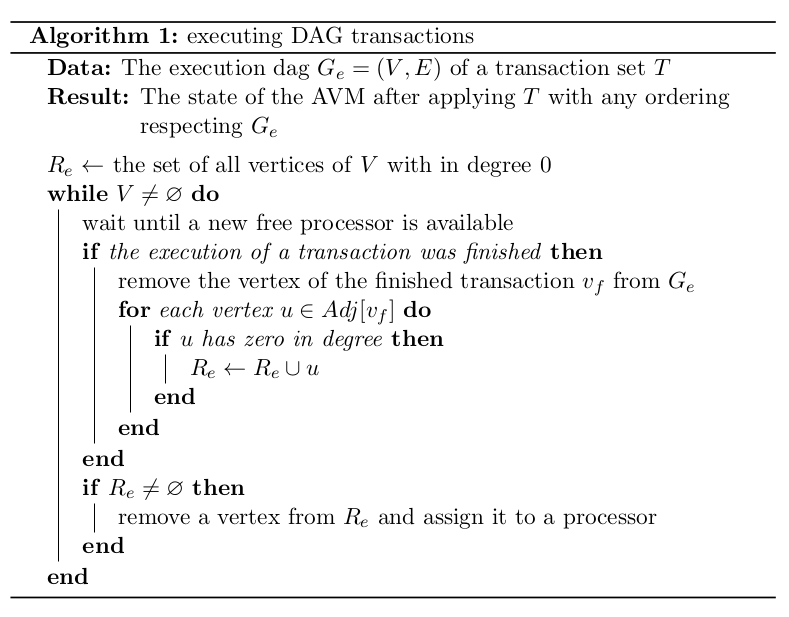
\includegraphics[width=17cm]{../img/Alg1s.png}
\begin{algorithm}
    \DontPrintSemicolon
    \SetKwData{Ready}{$R_e$}\SetKwData{V}{$v_f$}\SetKwData{Graph}{$G_e$}\SetKwData{Vertices}{$V$}\SetKwData
    {Txns}{$T$}
    \KwData{The execution dag $\Graph = (\Vertices,E)$ of transaction set \Txns}
    \KwResult{The state of the AVM after applying \Txns with any ordering respecting \Graph}
    \BlankLine
    \Ready $\gets$ the set of all vertices of \Vertices with in degree 0\;
    \While{$\Vertices \neq \varnothing$}
    {
        wait until a new free processor is available\;
        \If{the execution of a transaction was finished}
        {
            remove the vertex of the finished transaction \V from \Graph\;
            \For{each vertex $u \in Adj[\V]$}
            {
                \If{$u$ has zero in degree}
                {
                    $\Ready \gets \Ready \cup u$\;
                }
            }
        }
        \If{$\Ready \neq \varnothing$}
        {
            remove a vertex from \Ready and assign it to a processor\;
        }
    }
    \caption{executing DAG transactions}\label{alg:exec_dag}
\end{algorithm}

By replacing every undirected edge of a memory dependency graph with a directed edge in such a way that the
resulted graph has no cycles, we will obtain a valid execution DAG. Thus, from a memory dependency graph different
execution DAGs can be constructed with different levels of parallelization ability.

If we assume that we have unlimited number of processors and all transactions take equal time for executing, it
can be shown that by providing a minimal graph coloring to Algorithm~\ref{alg:gen_dag} as input, the resulted
DAG will be optimal, in the sense that it results in the minimum overall execution time.

%##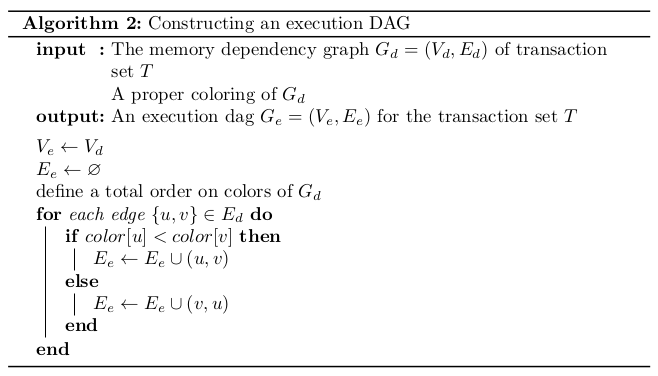
\includegraphics[width=17cm]{../img/Alg2s.png}
\begin{algorithm}
    \DontPrintSemicolon
    \SetKwData{Txns}{$T$}\SetKwData{Gd}{$G_d=(V_d,E_d)$}
    \SetKwInOut{Input}{input}\SetKwInOut{Output}{output}
    \Input{The memory dependency graph \Gd of transaction set \Txns\\A proper coloring of $G_d$}
    \Output{An execution dag $G_e=(V_e,E_e)$ for the transaction set \Txns}
    \BlankLine
    $V_e \gets V_d$\;
    $E_e \gets \varnothing$\;
    define a total order on colors of $G_d$\;
    \For{each edge $\{u,v\} \in E_d$}
    {
        \eIf{$color[u] < color[v]$}
        {
            $E_e \gets E_e \cup (u,v)$\;
        }{
            $E_e \gets E_e \cup (v,u)$\;
        }
    }
    \caption{Constructing an execution DAG}\label{alg:gen_dag}
\end{algorithm}

The block proposer is responsible for proposing an efficient execution DAG alongside his proposed block. This
execution DAG will determine the ordering of block transactions and help validators to validate transactions in
parallel. Since with better parallelization a block can contain more transactions, a proposer is incentivized enough
to find a good execution DAG for transactions.

\subsection{Memory Spooling}\label{subsec:spooling}

When two transactions are dependant and they are connected with an edge \((u,v)\) in the execution DAG,
the transaction \(u\) needs to be run before the transaction \(v\). However, if \(v\) does not read any
memory locations that \(u\) modifies, we can run \(u\) and \(v\) in parallel. We just need to make sure
\(u\) does not see any changes \(v\) is making in AVM memory. This can be done by appropriate versioning
of the memory locations which is shared between \(u\) and \(v\). We call this method \emph{memory spooling}.
After enabling memory spooling between two transactions the edge connecting them can be safely removed from the
execution DAG\@.

\subsection{Concurrent Counters}\label{subsec:concurrent-counters}

We know that in Argennon every transaction needs to transfer its proposed fee to the \texttt{feeSink} accounts
first. This essentially makes every transaction a reader and a writer of the memory locations which store the
balance record of the \texttt{feeSink} accounts. As a result, all transactions in Argennon will be dependant and
parallelism will be completely impossible. Actually, any account that is highly active, for example the account
of an exchange or a payment processor, could become a concurrency bottleneck in our system which makes all
transactions interacting with them dependant.

This problem can be easily solved by using a concurrent counter for storing the balance record of this type of
accounts. A concurrent counter is a data structure which improves concurrency by using multiple memory locations for
storing a single counter. The value of the concurrent counter is equal to the sum of its sub counters and it can
be incremented or decremented by incrementing/decrementing any of the sub counters. This way, a concurrent
counter trades concurrency with memory usage.

Algorithm~\ref{alg:CC} implements a concurrent counter which returns an error when the value of the counter
becomes negative.

%##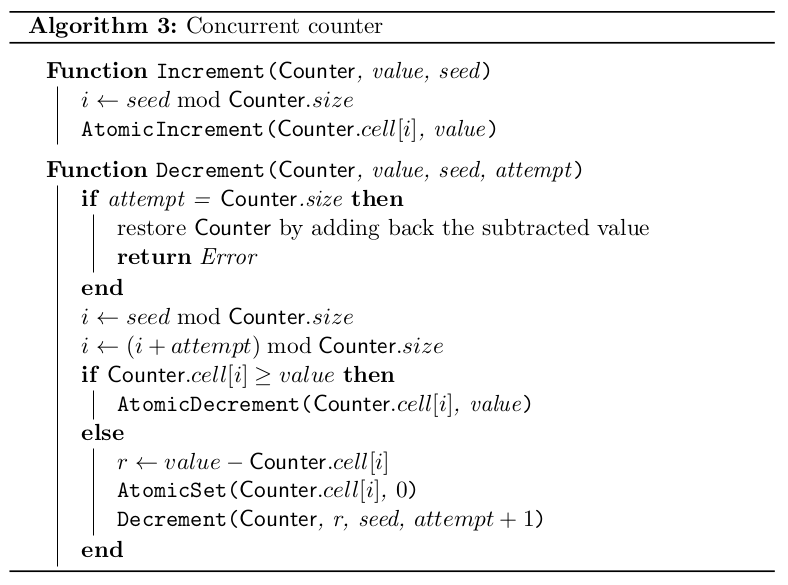
\includegraphics[width=17cm]{../img/Alg3s.png}
\begin{algorithm}
    \DontPrintSemicolon
    \SetKwData{CC}{Counter}
    \SetKwFunction{Inc}{Increment}\SetKwFunction{Dec}{Decrement}\SetKwFunction{AtomInc}{AtomicIncrement}
    \SetKwFunction{AtomDec}{AtomicDecrement}\SetKwFunction{AtomSet}{AtomicSet}\SetKwFunction{Get}{GetValue}
    \SetKwFunction{Acquire}{Lock.Acquire}\SetKwFunction{Release}{Lock.Release}
    \SetKwProg{Fn}{Function}{}{}
    \Fn{\Get{\CC}}
    {
        $s \gets 0$\;
    \Acquire{}\;
    \For{$i \gets 0$ \KwTo $\CC.size - 1$}
    {
        $s \gets s + \CC.cell[i]$\;
    }
    \Release{}\;
    \KwRet{s}\;
    }
    \BlankLine
    \Fn{\Inc{\CC, value, seed}}
    {
        $i \gets seed \bmod \CC.size$\;
    \AtomInc{$\CC.cell[i]$, value}\;
    }
    \BlankLine
    \Fn{\Dec{\CC, value, seed, attempt}}
    {
        \If {attempt = \CC.size}
        {
            restore \CC by adding back the subtracted value\;
            \KwRet{Error}\;
        }
        $i \gets seed \bmod \CC.size$\;
        $i \gets (i + attempt) \bmod \CC.size$\;
    \eIf {$\CC.cell[i] \geq value$}
    {
        \AtomDec{$\CC.cell[i]$, value}\;
    }{
        $r \gets value - \CC.cell[i]$\;
        \AtomSet{$\CC.cell[i]$, $0$}\;
        \Dec{\CC, r, seed, $attempt + 1$}\;
    }
    }
    \caption{Concurrent counter}\label{alg:CC}
\end{algorithm}

It should be noted that in a blockchain application we don't have concurrent threads and therefore we don't need
atomic functions. For usage in a smart contract, the atomic functions of this pseudocode can be implemented like
normal functions.

Concurrent counter data structure is a part of the AVM standard library, and any smart contract can use this data
structure for storing the balance record of highly active accounts.

\subsection{Memory Chunks}\label{subsec:memory-chunks}

In order to further increase the concurrency level of Argennon, we can divide the AVM memory into \emph{chunks}.
Each memory chunk can be persisted using a different ZK-EDB, hence having its own commitment. Then, the
consensus on new values of the commitment of any chunk can be achieved by a different voting committee.

If a transaction does not modify a memory chunk and in the transaction ordering of the block it comes after
any transaction which modifies that chunk, then the execution of that transaction is not needed for calculating
the new commitment of the chunk. Consequently, the voting committee of that memory chunk can safely ignore such a
transaction. The execution DAG of transactions can be used for finding and pruning these transactions as
we see in Algorithm~\ref{alg:prune_dag}.

%##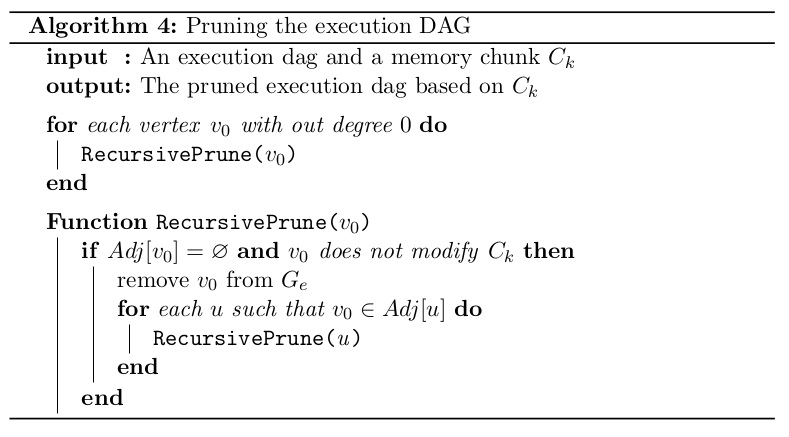
\includegraphics[width=17cm]{../img/Alg4s.png}
\begin{algorithm}
    \DontPrintSemicolon
    \SetKwData{V}{$v_0$}\SetKwData{Graph}{$G_e$}\SetKwData{Chunk}{$C_k$}\SetKwData{Txns}{$T$}
    \SetKwFunction{RPrune}{RecursivePrune}
    \SetKwProg{Fn}{Function}{}{}
    \SetKwInOut{Input}{input}\SetKwInOut{Output}{output}
    \Input{An execution dag \Graph and a memory chunk \Chunk}
    \Output{The pruned execution dag based on \Chunk}
    \BlankLine
    \For{each vertex \V with out degree $0$}
    {
        \RPrune{\V}\;
    }
    \BlankLine
    \Fn{\RPrune{\V}}
    {
        \If{$Adj[\V] = \varnothing$ {\bf and} \V does not modify \Chunk}
        {
            remove \V from \Graph\;
            \For{each $u$ such that edge $(u,\V)$ was in \Graph}
            {
                \RPrune{u}\;
            }
        }
    }
    \caption{Pruning an execution DAG}\label{alg:prune_dag}
\end{algorithm}

If we choose chunks in a way that most transactions only modify memory locations of one chunk,
likely many transactions of a block only need to be validated by one voting committee and can be validated in
parallel by different committees.

Because the voting committees are selected by random sampling, by choosing large enough samples we can make sure
that having multiple voting committees will not change the security properties of the Argennon agreement protocol.


\section{Smart Contract Oracle}\label{sec:smart-contract-oracle}

A smart contract oracle is a full AVM emulator that keeps a full local copy of AVM memory and can emulate AVM
execution without accessing a ZK-EDB. Smart contract oracles can be used for reporting useful information about
\texttt{avmCall} transactions such as accessed AVM heap or code area locations, exact amount of execution cost,
and so on.